\documentclass[a4paper,10pt]{article}
\usepackage[utf8]{inputenc}
\usepackage{tabularx}
\usepackage{amssymb}
\usepackage{hhline}
\usepackage{graphicx}
\usepackage{pstricks-add}
\newcommand{\intinf}{\int_{-\infty}^{\infty}}
\newcommand{\sumg}{\sum_{\gamma=0}^{2k}}
\newcommand{\spl}{\psi^{(k+1)}}
\usepackage{pgf,tikz}
%\usepackage[toc,page]{appendix}
%
% \usetikzlibrary{arrows}
\usepackage{rotating}
\usepackage{lscape}
\usepackage{epstopdf}
\newtheorem{theorem}{Theorem}[section]
\newtheorem{definition}{Definition}[section]
\usepackage{enumerate}% http://ctan.org/pkg/enumerate
\usepackage{pgf,tikz}
\usepackage{caption}
\usepackage{subcaption}
\usepackage{pdflscape}
\bibliographystyle{plain} % or: "chicago"
\usepackage{natbib} % a citation management package
\usepackage[utf8]{inputenc}
\usepackage{amsmath}
\usepackage{amsfonts}
\newtheorem{note}{Note}[section]
\usepackage{amssymb}
\usepackage{graphicx}
\usepackage{pstricks-add}
\usepackage{float}    
%\usepackage{multirow}
\newtheorem{proposition}{Proposition}
\newtheorem{lemma}{Lemma}
\setcounter{section}{0}
\usepackage{listings}
\author{Julia Docampo}
\newcommand{\xin}{x_{i-\frac 12}}
\newcommand{\xip}{x_{i+\frac 12}}
\usepackage{pgf,tikz}
\usetikzlibrary{arrows}
\usetikzlibrary{decorations.markings}
\usepackage{rotating}
\usepackage{lscape}
\usepackage{epstopdf}
\newtheorem{lema}{Lemma}[section]
\newtheorem{remark}{Remark}[section]
\newtheorem{corollary}{Corollary}[section]
%\usepackage{subfig}
%\newtheorem{proposition}{Proposition}[section]
\usepackage{enumerate}% http://ctan.org/pkg/enumerate
\newcommand*{\QEDA}{\hfill\ensuremath{\blacksquare}}%
\newcommand*{\QEDB}{\hfill\ensuremath{\square}}%
\usepackage{pgf,tikz}
\usetikzlibrary{positioning,arrows}
\usepackage{natbib}
\usepackage{etex}

\usepackage{color}
 
 \begin{document}
 
 
 \section{Introduction}
 \section{Defining the Problem}
 \section{The Algorithm}
 The methodology presented here attempts to approximate data to some user specified accuracy by applying an iterative scheme. 
In order to avoid solving the non-linear ``free knots'' problem, we propose the following approach: start with few (or minimal) number of control points and perform a curve fit solving the linear least-squares problem in order to find 
the points location. If the error is unacceptable, locate the knot span with highest squared error and insert a  new knot such that the error is split in halves. The process iterates until the desired tolerance is reached or it is not 
possible to introduce new suitable knots. We will discuss later what unsuitable knots mean. 

It is well known that as the number of control points approach the number of data points, the resulting approximating B-spline curve may present undesirable wiggles or end up producing artificial loops. Hence, we believe that 
a ``knot increasing'' iterative scheme is more stable than approximating the curve starting with a high number of control points and iterative remove the redundant ones. 
The usual approach for solving the least squares problem consists of a pre-stage that finds a suitable curve parametrization ($e.g.$, centripetal or chord-length)  ${t_j}_{j=1}^m$ that targets the $m$ data points and
then compute the knots location followed by finding the control points location that minimizes the error in the least squares sense. 
This curve discretization does observe the curve behavior between the evaluations $B(t_j)$ and $B(t_{j+1})$, where a ``parasitic'' loop may develop. If the local error is smaller than the tolerance, that 
curve zone will not be altered ($i.e.$, candidate for knot-removal in a knot decreasing iterative scheme) thus, producing undesirable results. Furthermore, knot spans that contain few $t$-values can end up having a dense control point area 
producing wiggles. Again, from the least-squares perspective, such wiggles do not exist as illustrated in Figure \ref{fig:wiggle_unif_vs_centr}.

\subsection{Linear Least Squares Approximation}
For a given a data set $\left\{X_i\right\}_{i=1}^m$ and $n>m$ control points, we look for the B-spline curve 
\begin{equation}
 C(u) = \sum_{i=0}^n N_{i,p} P_i,\quad u\in[0,1]
\end{equation}\label{eq:least_squares_equation1}
that approximates the data in the least squares sense:
$$
\sum _{k= 1}^{m-1}\left | X_k - C(t_k)\right|^2,\quad C(0)= X_0\ \text {and}\  C(1) = X_m.
$$
Let 
$$
 R_k = Q_k - N_{0,p}(t_k)Q_0 - N_{m,p}(t_k)Q_m,  k = 1,\ldots, m-1, 
$$
since the B-spline knots are fixed, minimizing equation \eqref{eq:least_squares_equation1} gives:
\begin{equation}\label{eq:linear_least_squares_solver}
 \sum_{i=1}^{n-1} \left(N_{\ell, p}(t_k)N_{i,p}(t_k)\right)P_i= \sum_{k=1}^{m-1}N_{\ell,[}(t_k)R_k, \quad \ell= 1\ldots, n-1
\end{equation}
 which produces a determined system of equations that can be solved applying any linear matrix solver. For more details, see \cite{nurbs_book}.
The limitations of this solver is that a suitable approximation assumes prior knowledge of the ``correct'' number of control points as well as the knot 
location. The algorithm presented next consists of inserting a new knot at 
each iteration followed by solving the new least squares problem applying equation \eqref{eq:least_squares_equation1}. 

\subsubsection{Knot Placement}\ref{sec:knot_placment}
A suitable knot sequence must ensure that each span contains at least one $t_k$ value so that \eqref{eq:linear_least_squares_solver} is well posed. 
We start with the minimum number of control points ( $n = p$) and the following knot sequence 
$U=\left\{0,\underbrace{\ldots}_{p-1},0,1,\underbrace{\ldots}_{p-1},1\right\}$. 
 At each iteration, we find the span with greatest squared error: 
 $$e_k = \frac{1}{N_k}\sum_{i=1}^{N_k} (C(t_i) - X_i)^2,\quad N_k = \# t_i\in [u_k, u_{k+1}), i=1,\ldots,m-1.$$
 At $e_k$, we look for the first $t_i$ such that $t_i >= e_k/2$ and we insert a knot $\tilde u = 0.5(t_i+t_{i+1}$. 
 \begin{remark}
  This knot choice ensures that every new span is non empty. 
 \end{remark}
In order to avoid concentrating too many control points at a particular zone, we introduce two additional 
constraints in our knot choice:
\begin{enumerate}
 \item The new knot has to be at a \emph{minimum} distance from the its neighboring knots which we have set to $1.e-06$. 
 \item The minimum $t_k$'s is set $>1$ initially and only when no more knots can be inserted (and the algorithm hasn't reached the desired tolerance) this condition is relaxed. 
\end{enumerate}

\subsubsection{The Algorithm}
Now that the least squares approach and knot placement have been discussed, we introduce the main algorithm and discuss implementation 
details. Once the desired tolerance is selected, we use the centripetal method in order to obtain a curve parametrization: 
\begin{align}
 d &= \sum_{k=1}^n \sqrt {| X_k-X_{k-1}|},\\
 t_0 &=0,\ t_m=1,\quad t_k = t_{k-1} + \frac{\sqrt{|X_k-X_{k-1}|}}{d},\quad k = 1,\ldots, m-1.
 \end{align}
This method has proven to be suitable for detecting curve features such as ``cusps'' \cite{}. 
\begin{note}
 If the initial number of control points is set $n > p$, we define the internal knots sequence proposed by proposed by \cite{}: 
  \begin{align}
  d &= \frac{m+1}{n-p+1} \Rightarrow i = int(j\cdot d),\quad \alpha = jd -i\\
  u_{p+j} &= (1-\alpha)u_{i-1} + \alpha u_i,\quad j = 1,\ldots,n-p.
 \end{align}
\end{note}

At each iteration, we solve \eqref{} and compute the global error. If we haven't reached the desired tolerance, 
we insert a knot as discussed in section \ref{sec:knot_placment} and find the new control points. If the 
new configuration has not significantly improved the previous iteration, we reject the knot and find the next worst error. 
 If all knots were found to be ``unsuitable'' we proceed with the best configuration, insert a new knot and tag its 
 value. Once a significant improvement has been found, we try to remove all the ``redundant'' points computed between the tagged knot and the 
 knot at valid iteration and when possible, the knots in between are removed. The algorithm stops when either the tolerance has reached, 
 the number of iterations have exceeded the maximum or when the approximation has stagnated: no new knot 
 produces a better approximation. The implementation steps are shown in Algorithm \ref{alg:solver}. 


\subsubsection{Computational Costs}
The methodology presented here attempts to avoid the ``free knot problem'' which involves solving a non-linear 
least squares solver. By sequentially increasing the number of control points together with a well chosen knot 
position, we can obtain a suitable approximation which relies on solving a linear system thus, avoiding excessive 
computational costs. Although we cannot prove that our knot position is optimal, it is designed to increase the accuracy 
 at where the maximum error in the least squares sense occur,
  thus it is in accordance with the minimization solver. 
  Furthermore as shown in the next section, our results reveal that this routine is suitable for 
   noisy data and does not ``destroy`` sharp features. 
   
   
\section{Results}
We begin by studying the performance of the solver on ''basic shapes`` as well as smooth data. 
Then we apply this routine on a level-set solution employed for studying ice formation and finally, we study 
 its behavior on nosy data. 
 
 \begin{table}
 \centering
  \begin{tabular}{|c| c| c|c |c|}
  \hline
 TOL&TIME (s)&Iters& NCP  & Error      \\ 
1.e-05&	0.006&	14&	18&	2.5e-06\\
1.e-06&	0.006&	17&	21&	9.6e-07\\
1.e-07&	0.009&	25&	29&	7.6e-08\\
\hline
   \end{tabular}
\caption{Results when approximating a 2D sine-wave $(t,\sin(t)), \ t\in[0,\pi]$ using 100 data points.}
 \end{table}

 \begin{table}
 \centering
  \begin{tabular}{||c c c c c ||c c c c c||}
  \hline
  \multicolumn{5}{||c||}{\textbf{Sphere Curve}} & \multicolumn{5}{c||}{\textbf{NACA}}\\
  \hline
 TOL    & TIME (s) & N  & N-Direct & RMS     & TOL    & TIME (s) & N  & N-Direct  & RMS     \\
 \hline
1.0e-05 & 2.20e-02 & 24	& 20 & 8.1e-06 & 1.0e-05 & 4.00e-02 & 12 & 19 & 9.7e-06\\
1.0e-06 & 1.40e-01 & 40	& 32 & 9.5e-07 & 1.0e-06 & 3.00e-01 & 27 & 35 & 8.8e-07\\
1.0e-07 & 2.73 & 73	& 54 & 1.0e-07 & 1.0e-07 & 4.70e-01 & 40 & 52 & 8.8e-08\\
\multicolumn{5}{||c||}{} & \multicolumn{5}{c||}{}\\
\multicolumn{5}{||c||}{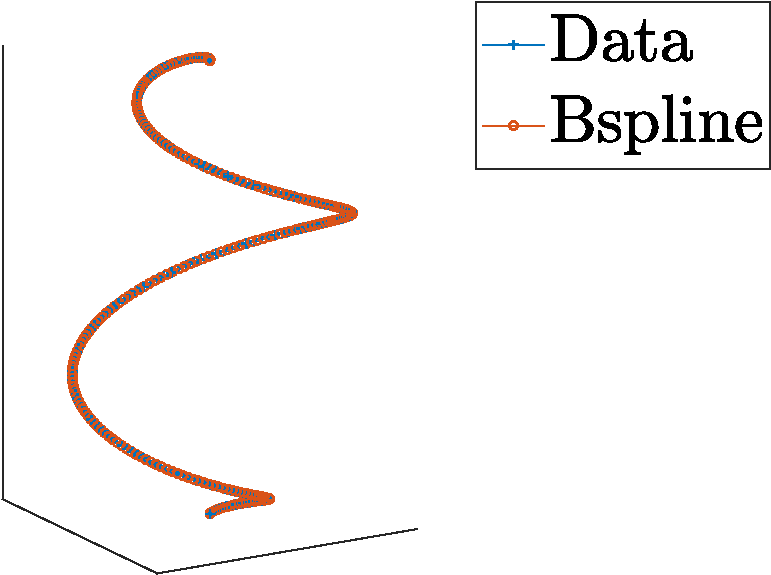
\includegraphics[width=0.45\textwidth]{snake-crop}}&
\multicolumn{5}{c||}{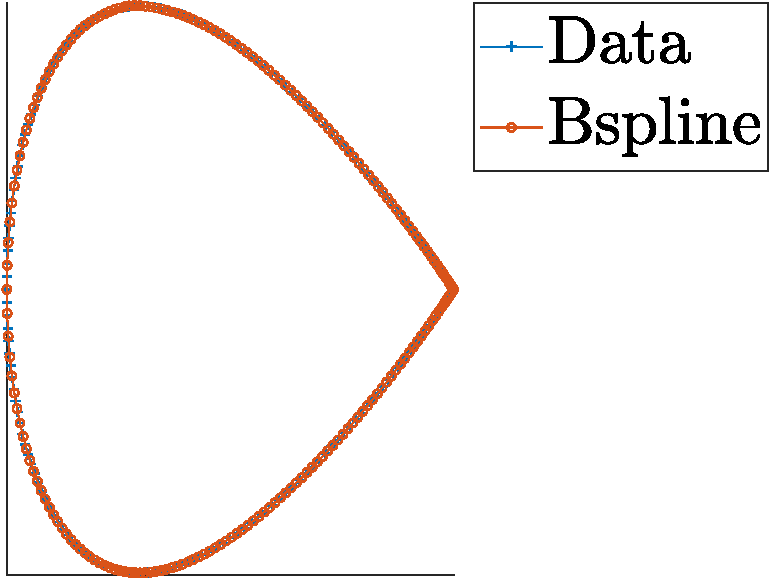
\includegraphics[width=0.45\textwidth]{naca27-crop} }\\
\hline
\end{tabular}
\caption{Results when approximating a curve moving along a sphere (see Figure \ref{fig:sphere_snake}) using 200 points.}
 \end{table}

 
 
 
 Figure \ref{} shows a helix obtained from \subsection{Basic Shapes Approximation}
 Consider
 
 



   
   
  





 
 
 

 
 
\end{document}

 